\documentclass{article}
\usepackage[utf8]{inputenc}
\usepackage{hyperref}
\usepackage[letterpaper, portrait, margin=1in]{geometry}
\usepackage{enumitem}
\usepackage{amsmath}
\usepackage{booktabs}
\usepackage{graphicx}

\usepackage{titlesec}

\titleformat{\section}
{\normalfont\Large\bfseries}{\thesection}{1em}{}[{\titlerule[0.8pt]}]
  
\title{Homework 9 Answers}
\author{Economics 7103}
\date{ }
  
\begin{document}
  
\maketitle

\begin{enumerate}
    \item See \ref{fig:hw9q1}.  It appears that when I wrote the simulation that I accidentally included a common shock for year 3, but even though the graph is unrealistic, we can see the rollout of the second set of treatments.
    \item See column 1 of table \ref{tab:didtable}.
    \item See column 2 of table \ref{tab:didtable}.  Note the estimates did not change, but the standard errors did change due to clustering two way.s
    \item Now, there is no ``clean control'' or never-treated group.  The TWFE estimator will give the weighted average of all the possible DIDs.
    \item The command reports that out of 924 ATTs, 600 receive a positive weight and 324 receive a negative weight.
    \item See column 3 of table \ref{tab:didtable}.  It turns out that the command is not written in a standard way so that you can use \verb!outreg2! to easily store the results.  Instead, I wrote a program around the command that would output the results into Stata's e-class.  Finally, I used \verb!esttab! instead of \verb!outreg2! to create the tables.  See the code.
    \item Now, all 324 weights are positive.  This is because dropping the last month leaves us in a ``standard'' DID setting where there is only one treatment time.
\end{enumerate}

\begin{figure}
    \centering
    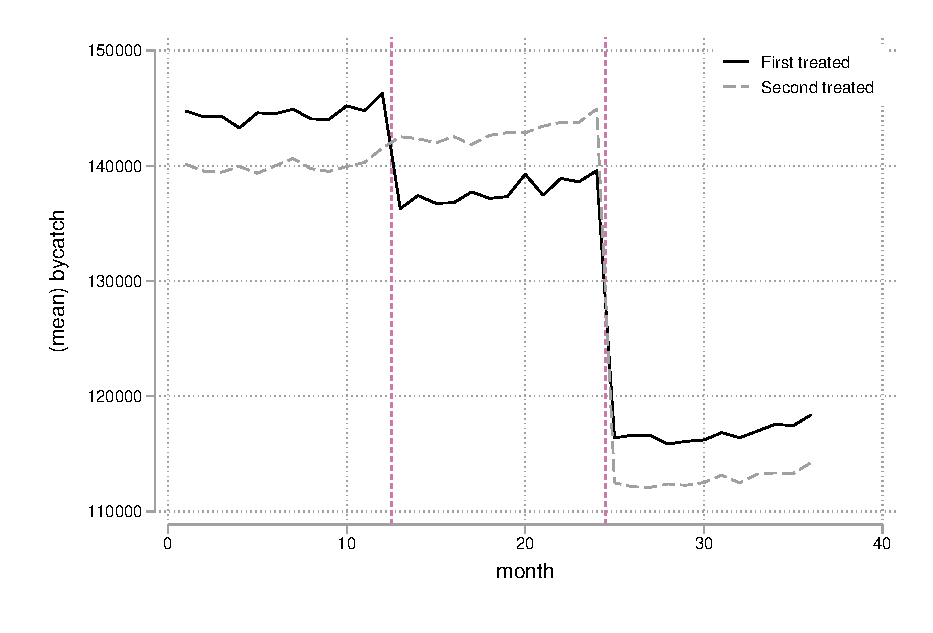
\includegraphics{hw9q1.eps}
    \caption{Fish bycatch over time by group}
    \label{fig:hw9q1}
\end{figure}

\begin{table}[]
    \centering
    {
\def\sym#1{\ifmmode^{#1}\else\(^{#1}\)\fi}
\begin{tabular}{l*{3}{c}}
\hline\hline
                    &\multicolumn{1}{c}{(1)}&\multicolumn{1}{c}{(2)}&\multicolumn{1}{c}{(3)}\\
                    &\multicolumn{1}{c}{xtreg}&\multicolumn{1}{c}{reghdfe}&\multicolumn{1}{c}{DID\_M}\\
\hline
Treatment           &     -6424.0\sym{*}  &     -6424.0\sym{*}  &     -8155.3\sym{**} \\
                    &     (-2.15)         &     (-2.21)         &     (-3.24)         \\
[1em]
Shrimp              &       1.792\sym{***}&       1.792\sym{***}&                     \\
                    &     (11.13)         &      (9.89)         &                     \\
[1em]
Salmon              &      -6.710\sym{***}&      -6.710\sym{***}&                     \\
                    &    (-13.59)         &     (-9.35)         &                     \\
\hline
N                   &        1800         &        1800         &          50         \\
\hline\hline
\multicolumn{4}{l}{\footnotesize \textit{t} statistics in parentheses}\\
\multicolumn{4}{l}{\footnotesize \sym{*} \(p<0.05\), \sym{**} \(p<0.01\), \sym{***} \(p<0.001\)}\\
\end{tabular}
}

    \caption{Caption}
    \label{tab:didtable}
\end{table}

\end{document}